% To define the scope of the product we can use ``The World \& Machine'' approach by M. Jackson and P. Zave.
% We can define the real world entities that interact with the system (the World), the entities that belong to the system (the Machine) and the shared phenomena (the intersection of the two other sets).

The \textit{The World and the Machine} approach is used in defining the scope of the project.
By defining the real world entities that interact with the system and the properties of the system itself we can determine the intersection between the two sets: the \textit{shared phenomena}.

\begin{figure}[H]
	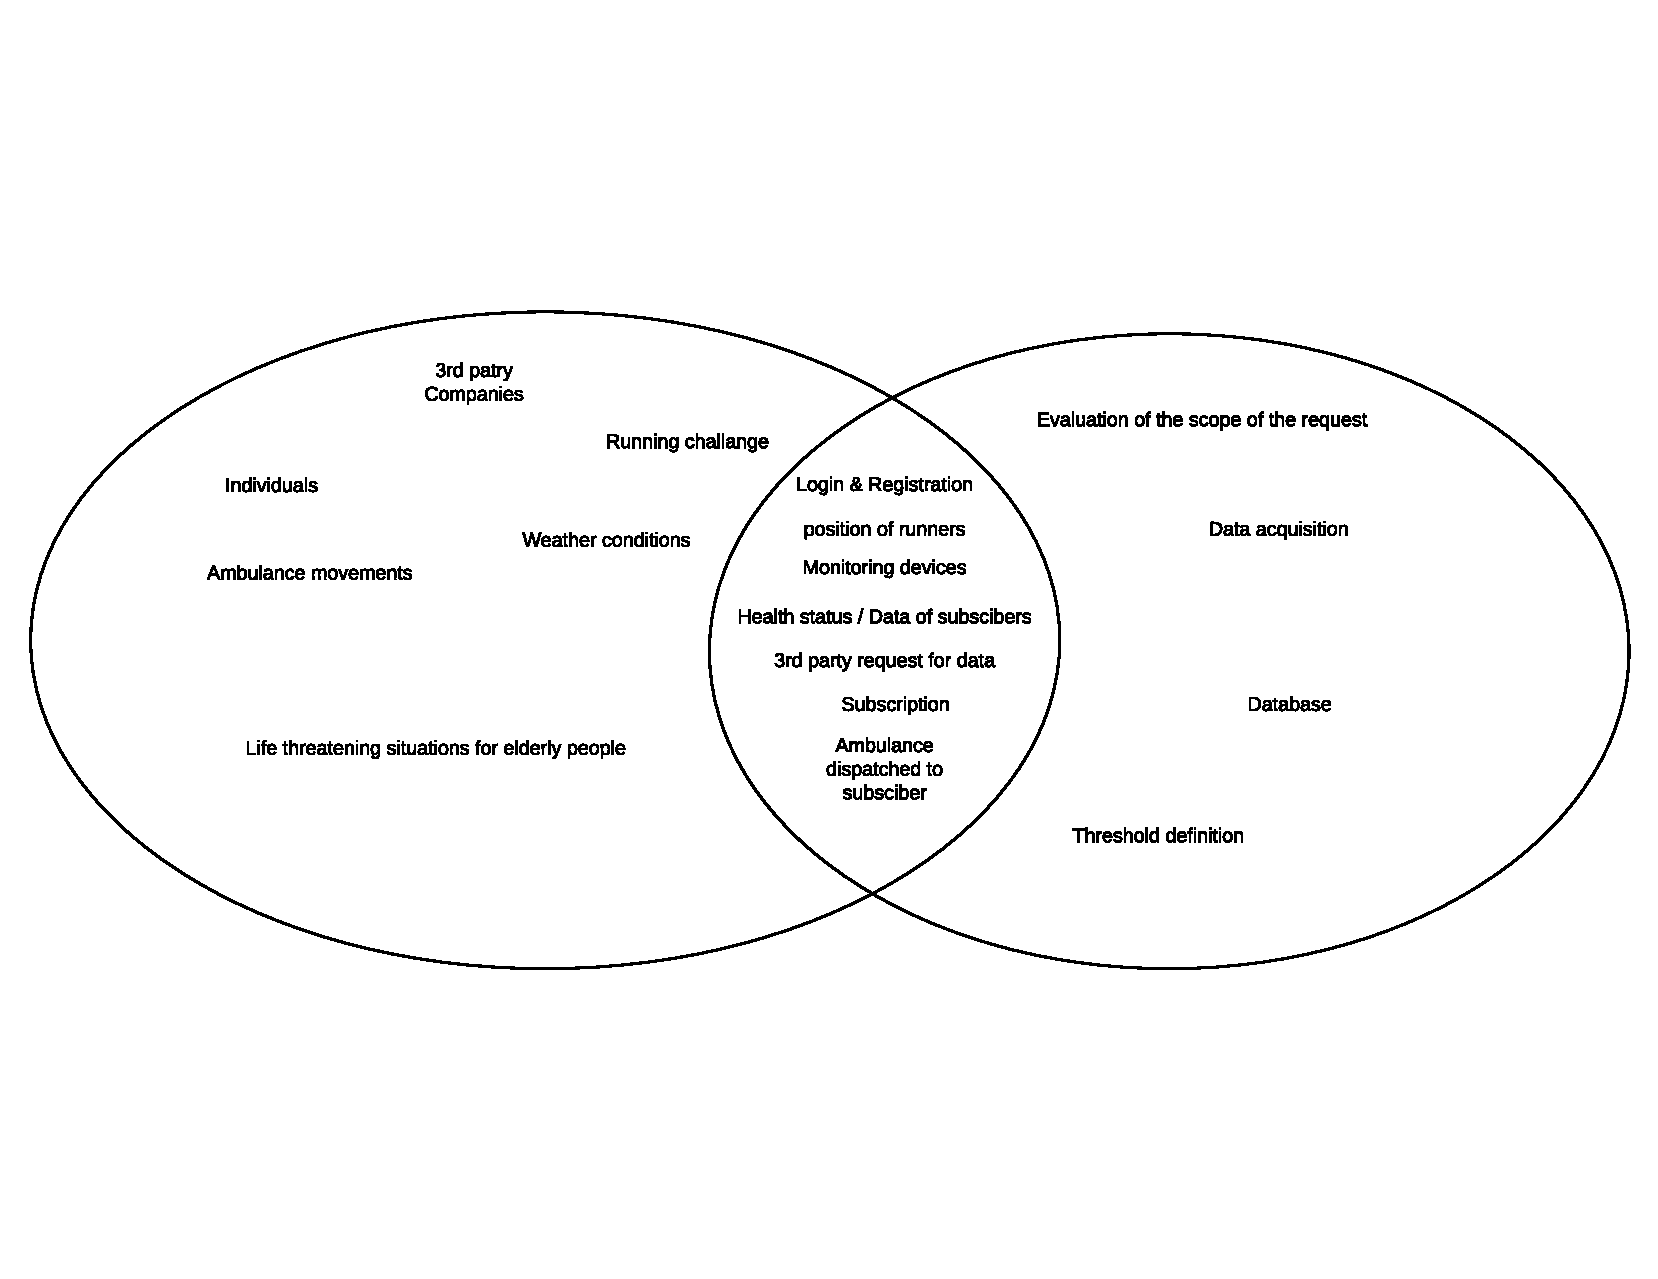
\includegraphics[width=\textwidth,height=\textheight,keepaspectratio]{assets/twatm.pdf}
	\caption{The World and the Machine diagram}
	\label{fig:TWATM}
\end{figure}

The system-to-be uses 4 components with different roles in order to function:
\begin{itemize}
    \item \textbf{Data4Help SmartWatch App}: Acquires the data from the smartwatch sensors (heart rate, sleep quality, position, phisical activities) and sends them via Bluetooth to the Data4Help Mobile App.
    \item \textbf{Data4Help Mobile App}: Gathers data from the smartwatch, shows various statistics, and sends them to the Data4Help Core Database. Each user can choose which service he would like to subscribe to.
    Moreover, it allows the organizers of a running event to define the path of the race and lets the spectators to see the position of all runners of a particular race on a map.
    \item \textbf{Data4Help Website}: Enables third-party companies to request data, either anonymous or user-specific.
    \item \textbf{Data4Help Core}: is intended to connect all other components together providing the logic of the application. It is also responsible for the acceptance of all third-parties requests of data. It also evaluates health status of individuals deciding whether it is at risk or not.
\end{itemize}

The list below shows the main goals the system should be able to accomplish:

\begin{itemize}
    \item \textbf{G1}: The system should be able to show acquired data via the Mobile App and the Website.
    \item \textbf{G2}: The system should allow users to register.
    \item \textbf{G3}: The system should allow companies to register.
    \item \textbf{G4}: The system should allow registered companies to request data from an anonymous group of individuals, only if individuals in the group are more than 1000.
    \item \textbf{G5}: The system should allow registered companies to request data from an individual person, only if individuals accept the request.

    \item \textbf{G6}: The system should let companies to be able to pay through the system in order to buy data queries/subscribe to plans.

    \item \textbf{G7}: The system should allow a company to subscribe to new data and receive them as soon as they are produced.
    \item \textbf{G8}: The system should be able to store user's health parameters.
    \item \textbf{G9}: The system should be able to react to the lowering of the health parameters below threshold in less than 5 seconds and send the position of the person to the ambulance system. 
    
    \item \textbf{G10} The system should allow run organizers to register.
    \item \textbf{G11} If a run organizer is registered, it can define a run i.e. it can define the path that the participants should follow.
    \item \textbf{G12} A user should be able to enroll for a run.
    \item \textbf{G13} Spectators of a run should be able to see each participant's position on a map.
    \item \textbf{G14} Individuals should be able to log-in.
    \item \textbf{G15} Companies should be able to log-in.
    \item \textbf{G16} Run organizers should be able to log-in.

\end{itemize}

%A health data aggregator app that gives the user the ability to monitor all 

%is intended to offer all the functionalities of the service to the individuals, including heart rate monitoring, sleep monitoring



